\documentclass{article}
\usepackage[a4paper,inner=1.5cm,outer=1.5cm,top=2cm,bottom=0.5cm]{geometry} 
\newcommand{\myhash}{\raisebox{\depth}{\#}}
\usepackage{multicol}
\usepackage{tikz}
\usepackage{amsmath}
\usepackage{mathtools}
\usepackage{gensymb}
\usepackage{pgfplots}
\usepackage{cancel}
\usetikzlibrary{intersections}
\usetikzlibrary{intersections,calc,angles,quotes}
\usetikzlibrary{calc,angles,positioning,intersections,quotes,decorations.markings}
\usepackage{tkz-euclide}
\usetikzlibrary{backgrounds}
\usetikzlibrary{calc,through}
\usetikzlibrary{angles}
\usetikzlibrary{fadings}
\usetikzlibrary{shapes.geometric}
\usepackage{draftwatermark}
\usepackage{mathptmx} 
\SetWatermarkText{Mathema Shukur}
\SetWatermarkFontSize{3 cm}
\usepackage[utf8]{inputenc}
\usepackage{fontspec}
\setlength{\columnsep}{2cm}
\setmainfont{[Kalpurush.ttf]}
\newfontface{\en}{[Arial.ttf]}
\usetikzlibrary{shapes.geometric, arrows}
\tikzstyle{startstop} = [draw, ellipse,minimum width=3cm, minimum height=1cm,text centered, draw=black]
\tikzstyle{io} = [trapezium, trapezium left angle=70, trapezium right angle=110, minimum width=3cm, minimum height=1cm, text centered, draw=black]
\tikzstyle{process} = [rectangle, minimum width=3cm, minimum height=1cm, text centered, draw=black]
\tikzstyle{decision} = [diamond, minimum width=3cm, minimum height=1cm, text centered, draw=black]
\tikzstyle{connector} = [circle, radius=1cm, text centered, draw=black]
\tikzstyle{arrow} = [thick,->,>=stealth]
\tikzstyle{line} = [draw, -latex']  
\begin{document} 
	\Large
	যাদের জন্যে প্রযোজ্যঃ  	\textcolor{black}{একাদশ ও দ্বাদশ শ্রেণীর শিক্ষার্থী} \\
	বিষয়ঃ \textcolor{black}{উচ্চতর গণিত ১ম পত্র} \\
	অধ্যায়ঃ \textcolor{black}{৩-সরলরেখা }\\ 
	Subtopicঃ \textcolor{black}{বিভক্তকারী বিন্দুর স্থানাঙ্ক }\\	
	(1) রাজশাহী বোর্ড-২০১৯\\
$P(4,3)$ ও $Q(-8,-5)$ বিন্দুর সংযোগ রেখাকে x-  অক্ষ যে অনুপাতে বিভক্ত করে তা বের কর।  \\
	\\
	 (2) বরিশাল বোর্ড-২০১৭\\
$(1,2)$ এবং  $(3,6)$ বিন্দুদ্বয়ের সংযোজক রেখাকে যে বিন্দু $2:3$ অনুপাতে অন্তর্বিভক্ত করে তাঁর স্থানাঙ্ক নির্ণয় কর।  \\
	\\
		(3) কুমিল্লা বোর্ড-২০১৭\\
$A(1,-2)$ এবং  $B(-8,1)$ বিন্দুদ্বয়ের সংযোজক রেখা BA কে  যে বিন্দু $2:1$ অনুপাতে অন্তর্বিভক্ত করে তাঁর স্থানাঙ্ক নির্ণয় কর।  \\
\\
	(4) রাজশাহী বোর্ড-২০১৯\\
 $x+3y+3=0$ রেখাটি দ্বারা অক্ষদ্বয়ের খন্ডিত অংশের মধ্যবিন্দুর স্থানাঙ্ক নির্ণয় কর। \\
 \\
 (5) দিনাজপুর বোর্ড-২০১৯\\ 
 $x-2y-5=0$ ও $2x+4y-1=0$ রেখাদ্বয়ের ছেদ বিন্দু নির্ণয় কর।\\
 \\ 
	যাদের জন্যে প্রযোজ্যঃ  	\textcolor{black}{একাদশ ও দ্বাদশ শ্রেণীর শিক্ষার্থী} \\
বিষয়ঃ \textcolor{black}{উচ্চতর গণিত ১ম পত্র} \\
অধ্যায়ঃ \textcolor{black}{৩-সরলরেখা }\\ 
Subtopicঃ \textcolor{black}{দুইটি বিন্দুর মধ্যবর্তী দূরত্ব }\\	
\\
(1) রাজশাহী বোর্ড-২০১৭\\
y-  অক্ষ এবং $(k,4)$  বিন্দু থেকে $A(2,4)$ বিন্দুর দূরত্ব সমান হলে k  এর মান নির্ণয় কর।\\
\\
(2) CU-2010-2011\\
y-  অক্ষ এবং $(7,2)$  বিন্দু থেকে $(a,5)$ বিন্দুর দূরত্ব সমান হলে a  এর মান নির্ণয় কর।\\
\\
(3) CU-13-14\\
x-  অক্ষ এবং $(-5,-7)$  বিন্দু থেকে $(4,k)$ বিন্দুর দূরত্ব সমান হলে k  এর মান নির্ণয় কর।\\
\\
(4) কুমিল্লা বোর্ড-২০১৯\\
$x+y-2=0$ রেখাটির মূলবিন্দু হতে লম্ব দূরত্ব নির্ণয় কর।\\
\\
(5) চট্রগ্রাম বোর্ড-২০১৯\\
$4y=3(x-4)$ এবং $4y=3(x-1)$ রেখা দুইটির মধ্যবর্তী লম্ব দূরত্ব নির্ণয় কর।   
\\
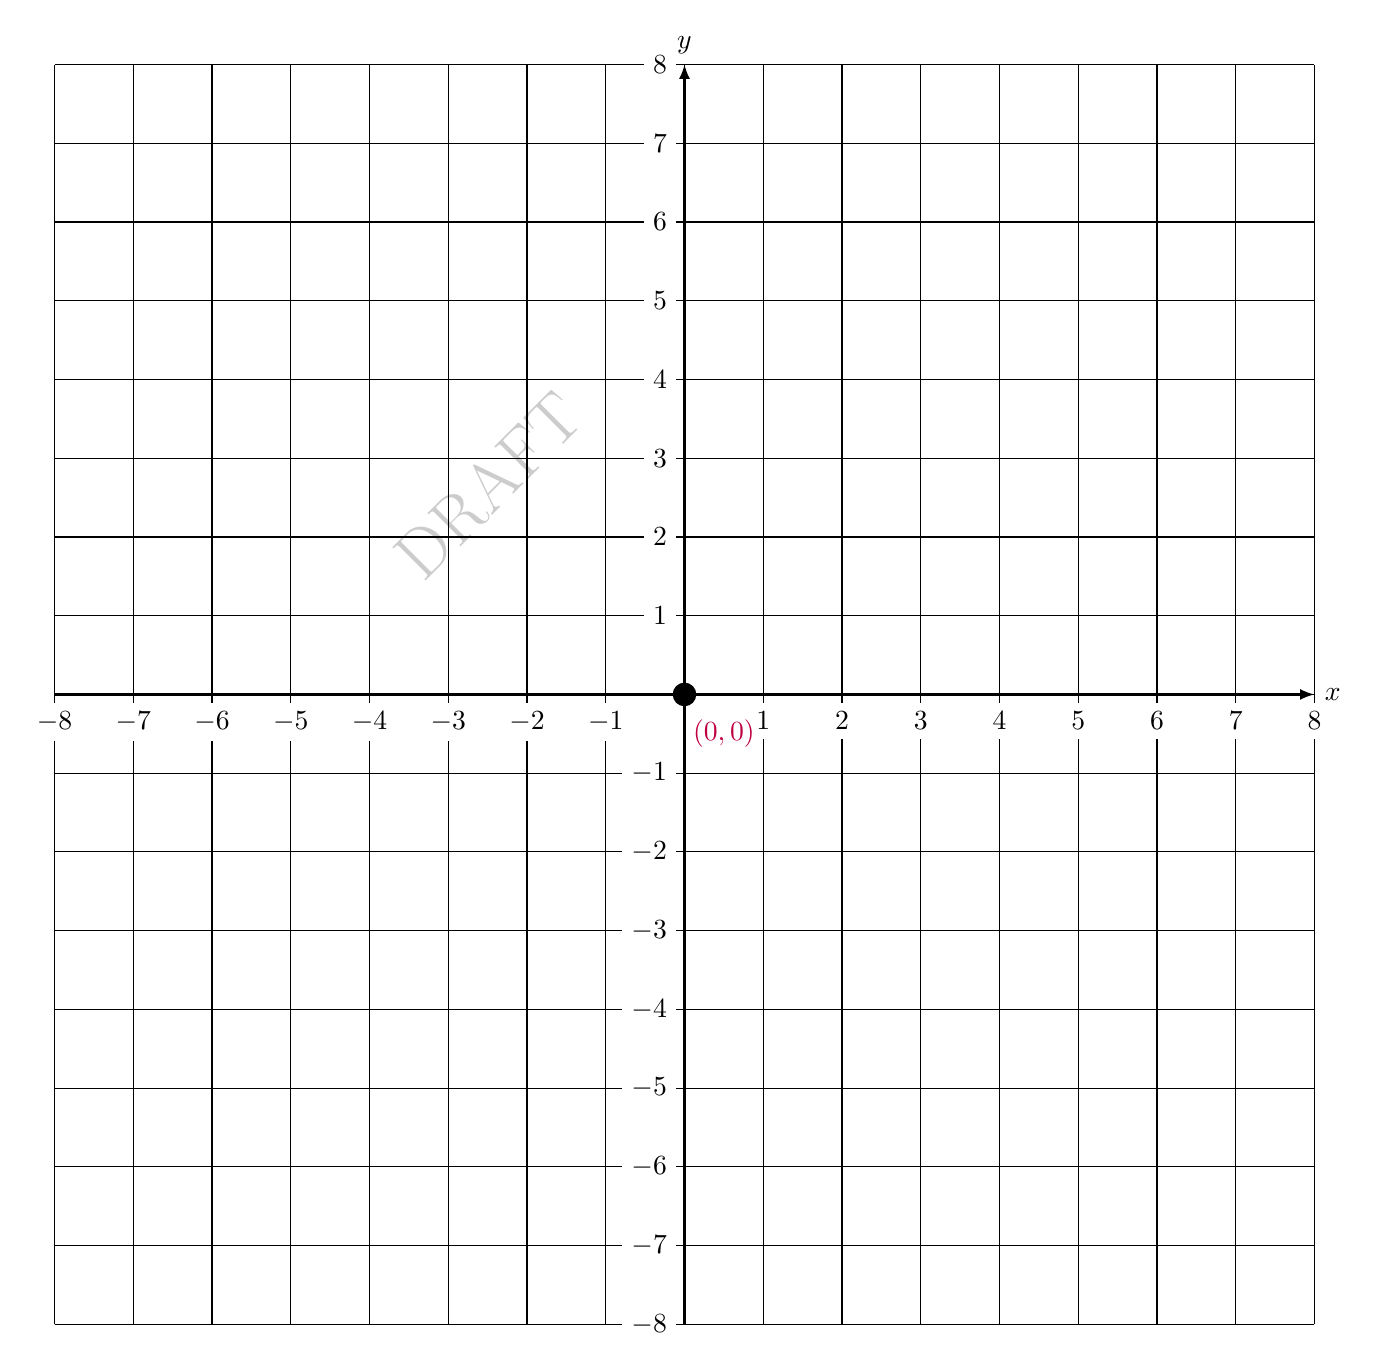
\begin{tikzpicture}[transform shape,scale=1]
	\draw (-8,-8) grid (8,8);
	\draw [-latex,thick](-8,0) -- (8,0) node[right] {$x$} coordinate(x axis);
	\foreach \x in {-8,-7,-6,-5,-4,-3,-2,-1,1,2,3,4,5,6,7,8}
	\draw (\x,0.1) -- (\x,-0.1) node [fill=white,below] {$\x$};
	\draw [-latex,thick](0,-8) -- (0,8) node[above] {$y$} coordinate(y axis);
	\foreach \y in {-8,-7,-6,-5,-4,-3,-2,-1,1,2,3,4,5,6,7,8}
	\draw (0.1,\y) -- (-0.1,\y) node [fill=white,left] {$\y$};
	\fill[black] (0,0) circle (1.5 mm);
	\node at (0.5,-0.5) {$\textcolor{purple}{(0,0)}$};
\end{tikzpicture}
\\ 
The cartesian coordinate system is a branch of mathematics that tells about how to represent a point uniquely in the n-dimensional coordinate plane. The theory of the cartesian system was proposed by a French philosopher and mathematician called Rene Descartes in the 17th century. This cartesian coordinate system provided the relationship between Euclidean geometry and algebra, which has revolutionized the study of mathematics. The cartesian coordinate system is the foundation of analytical geometry and helps in the representation of lines, curves, geometric figures in the n-dimensional plane. Let us learn more about the cartesian system and the terms associated with it.\\
\\
The coordinates are always written in a certain order:
\\
the horizontal distance first,
then the vertical distance.
This is called an "ordered pair" (a pair of numbers in a special order)
\\
And usually the numbers are separated by a comma, and parentheses are put around the whole thing like this:\\
\\
Abscissa and Ordinate
You may hear the words "Abscissa" and "Ordinate" ... they are just the x and y values:
\\
Abscissa: the horizontal ("x") value in a pair of coordinates: how far along the point is
Ordinate: the vertical ("y") value in a pair of coordinates: how far up or down the point is\\
\\
Four Quadrants
When we include negative values, the x and y axes divide the space up into 4 pieces:\\
\\
Example: The point "C" (-2,-1) is 2 units along in the negative direction, and 1 unit down (i.e. negative direction).
\\
Both x and y are negative, so that point is in "Quadrant III"
\\
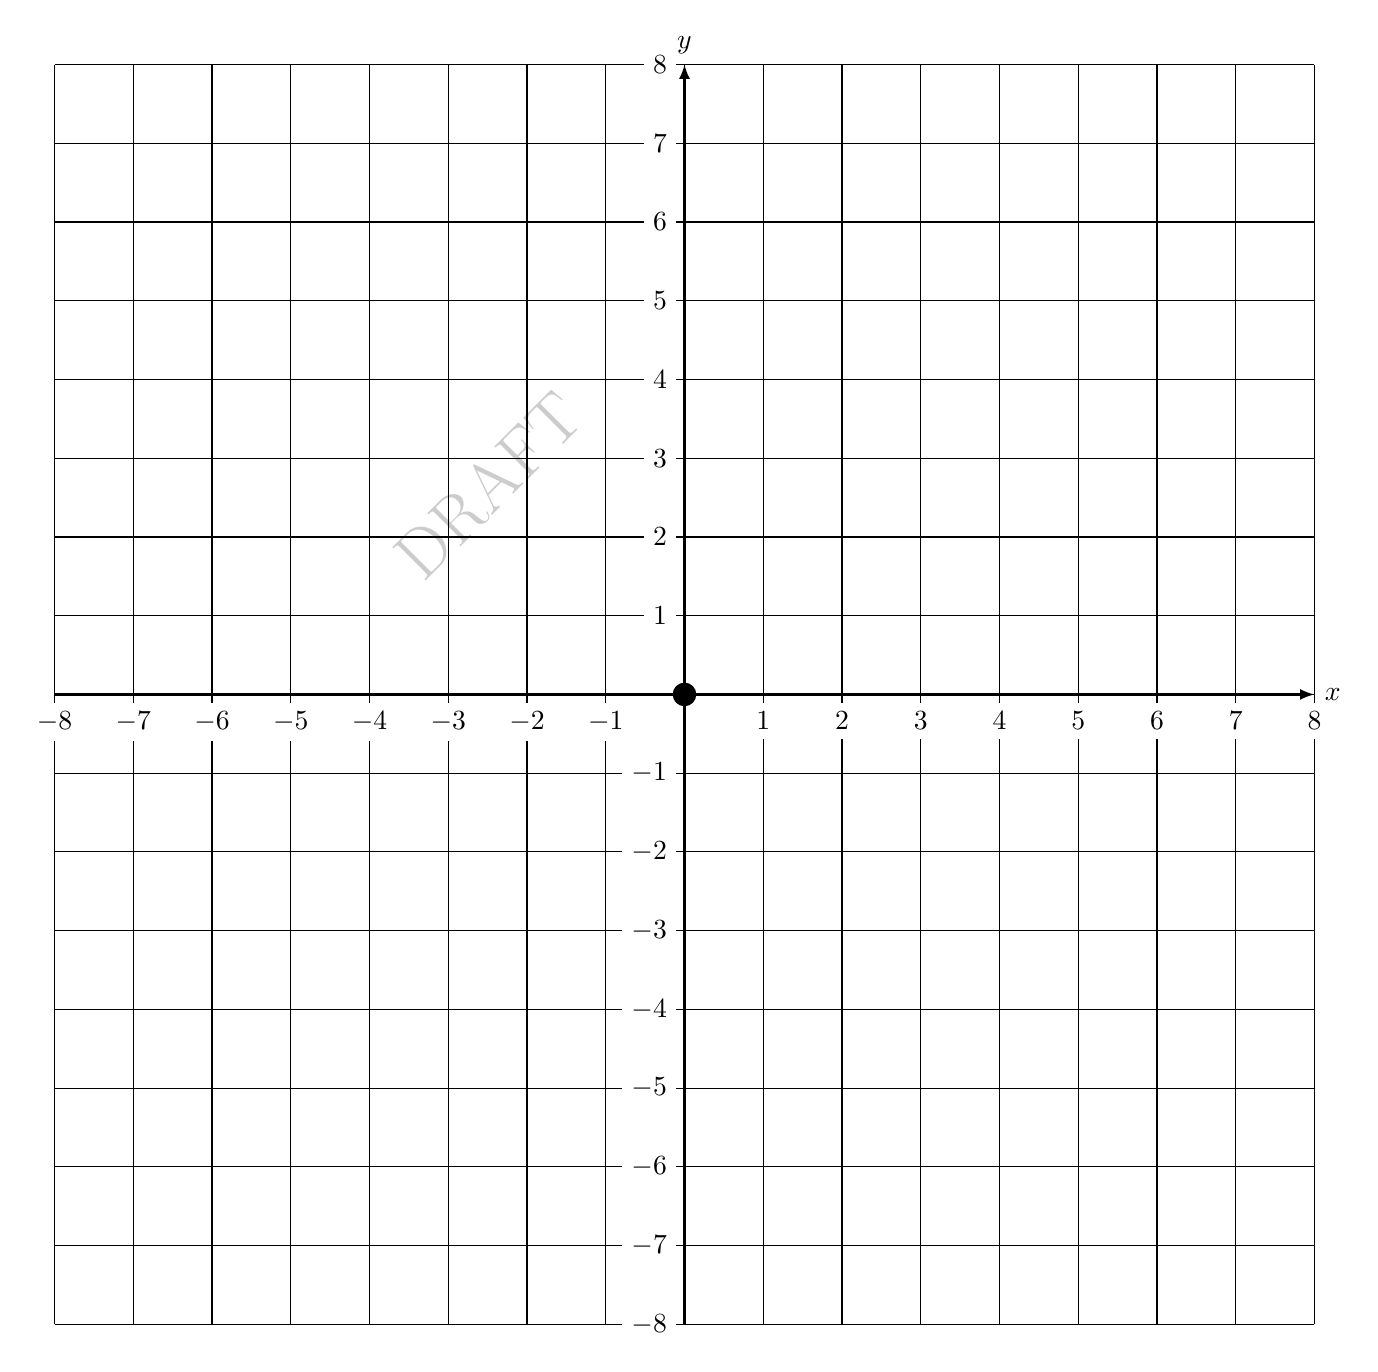
\begin{tikzpicture}[transform shape,scale=1]
	\draw (-8,-8) grid (8,8);
	\draw [-latex,thick](-8,0) -- (8,0) node[right] {$x$} coordinate(x axis);
	\foreach \x in {-8,-7,-6,-5,-4,-3,-2,-1,1,2,3,4,5,6,7,8}
	\draw (\x,0.1) -- (\x,-0.1) node [fill=white,below] {$\x$};
	\draw [-latex,thick](0,-8) -- (0,8) node[above] {$y$} coordinate(y axis);
	\foreach \y in {-8,-7,-6,-5,-4,-3,-2,-1,1,2,3,4,5,6,7,8}
	\draw (0.1,\y) -- (-0.1,\y) node [fill=white,left] {$\y$};
	\fill[black] (0,0) circle (1.5 mm);
\end{tikzpicture}
\\
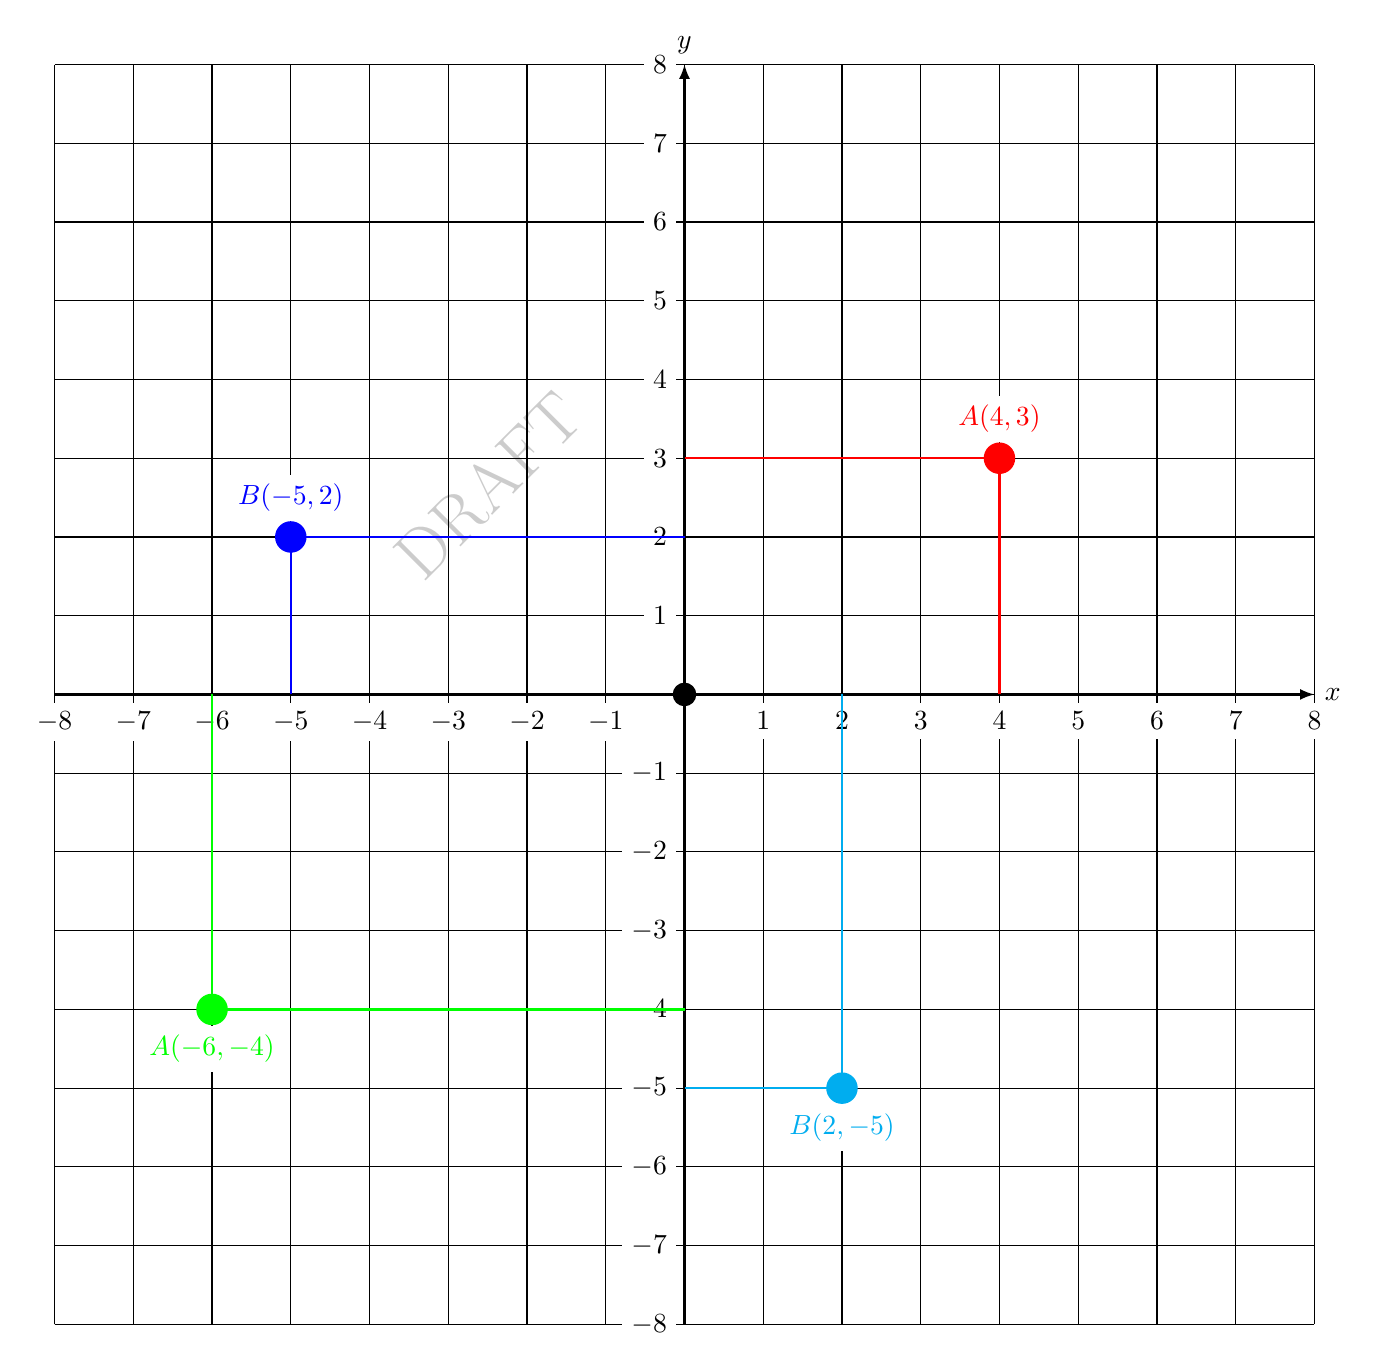
\begin{tikzpicture}[transform shape,scale=1]
	\draw (-8,-8) grid (8,8);
	\draw [-latex,thick](-8,0) -- (8,0) node[right] {$x$} coordinate(x axis);
	\foreach \x in {-8,-7,-6,-5,-4,-3,-2,-1,1,2,3,4,5,6,7,8}
	\draw (\x,0.1) -- (\x,-0.1) node [fill=white,below] {$\x$};
	\draw [-latex,thick](0,-8) -- (0,8) node[above] {$y$} coordinate(y axis);
	\foreach \y in {-8,-7,-6,-5,-4,-3,-2,-1,1,2,3,4,5,6,7,8}
	\draw (0.1,\y) -- (-0.1,\y) node [fill=white,left] {$\y$};
	\fill[black] (0,0) circle (1.5 mm);
	\fill[red] (4,3) circle (2 mm);
	\fill[blue] (-5,2) circle (2 mm);
	\fill[green] (-6,-4) circle (2 mm);
	\fill[cyan] (2,-5) circle (2 mm);
	\node[fill=white,above] at (4,3.2) {$\textcolor{red}{A(4,3)}$};
	\node[fill=white,above] at (-5,2.2) {$\textcolor{blue}{B(-5,2)}$};
	\node[fill=white,below] at (-6,-4.2) {$\textcolor{green}{A(-6,-4)}$};
	\node[fill=white,below] at (2,-5.2) {$\textcolor{cyan}{B(2,-5)}$};
	\draw[thick,red] (4,0)--(4,3);
	\draw[thick,red] (0,3)--(4,3);
	\draw[thick,blue] (-5,0)--(-5,2);
	\draw[thick,blue] (0,2)--(-5,2);
	\draw[thick,green] (-6,0)--(-6,-4);
	\draw[thick,green] (0,-4)--(-6,-4);
	\draw[thick,cyan] (2,0)--(2,-5);
	\draw[thick,cyan] (0,-5)--(2,-5);
\end{tikzpicture}
\\
the distance from a point to the vertical or y -axis, measured parallel to the horizontal or x -axis; the x -coordinate.\\
\\
the number in an ordered pair of numbers (as y in (x, y)) that gives the location of a point along the y-axis
called also y-coordinate\\  
\end{document}